\documentclass[11pt]{article}


\usepackage{amssymb, amsmath, verbatim, amsthm,url, multirow,fullpage,mathtools, appendix}
\usepackage{longtable, rotating,makecell,array}
\usepackage[aligntableaux=top]{ytableau}


\setlength{\parindent}{0pt}
\setlength{\parskip}{1.5ex plus 0.5ex minus 0.2ex}


%***************************
%Frontmatter Table of contents
%***************************
% Annotations
%xypic packages
%WLD tkx program
%Useful numeric rings and fields
%Other useful mathematical operations and functions
%Equation display shortcuts
%Shortcuts for frequently used special characters
%Theorem environments
%***************************

%*****************
% Annotations
\usepackage{soul}
\usepackage[colorinlistoftodos,textsize=footnotesize]{todonotes}
\newcommand{\hlfix}[2]{\texthl{#1}\todo{#2}}
\newcommand{\hlnew}[2]{\texthl{#1}\todo[color=green!40]{#2}}
\newcommand{\sanote}{\todo[color=violet!30]}
\newcommand{\note}{\todo[color=green!40]}
\newcommand{\newstart}{\note{The inserted text starts here}}
\newcommand{\newfinish}{\note{The inserted text finishes here}}
\setstcolor{red}
%***************************


%*****************
%xypic packages
\usepackage[all]{xy}
\xyoption{poly}
\xyoption{arc}
%*****************

%*****************
%%% WLD drawing 

\usetikzlibrary{calc} 
\usetikzlibrary{decorations.pathmorphing} % to get the wiggly propagator lines
\usetikzlibrary{bending} % to fix the arrow tips on bent lines
\usetikzlibrary{patterns} % for shading the Le diagrams in section 4

\newcommand{\leplus}{\Large $+$}
\newcommand{\lezero}{\Large $0$}

\newcommand{\leplusbold}[1][black]{%
  \tikz\draw[#1,line width=1.5pt,scale = 0.35,line cap = round] (0,0) -- (1,0)(0.5,0.5) -- (0.5,-0.5);
}


\definecolor{light-gray}{gray}{0.6}

% some propagator styles
\tikzstyle{propagator}=[decorate,decoration={snake,amplitude=0.8mm}]
\tikzstyle{smallpropagator}=[decorate,decoration={snake,segment length=3mm,amplitude=0.5mm}]

% for highlighting regions of a diagram edge
\tikzstyle{linehighlight}=[blue,line width = 3pt,line cap = round, draw opacity = 0.5]

% these two for drawing partial propagators
\tikzstyle{firstdash}=[dashed,line cap=round, dash pattern=on 2pt off 1pt]
\tikzstyle{seconddash}=[dashed,line cap=round, dash pattern=on 0.5pt off 1pt]
\tikzstyle{smalldash}=[dashed,line cap=round, dash pattern=on 1.5pt off 2pt]


 % used for showing which propagator assigns to which vertex in the last section
\pgfmathsetmacro{\arrowangle}{90}
\tikzstyle{propassignment} = [->,shorten >=2pt,thick]


% to draw a (full) WLD; \drawWLD{8}{2} is a circle of radius 2 with 8 marked points
\newcommand{\drawWLD}[2]{

\pgfmathsetmacro{\n}{#1}
\pgfmathsetmacro{\radius}{#2}
\pgfmathsetmacro{\angle}{360/\n}
\draw (0,0) circle (\radius);
    \foreach \i in {1,2,...,\n} {
      \draw (\angle*\i:\radius) node {$\bullet$};
       %\pgfmathsetmacro{\x}{\angle*\i}
       %\draw[-,shorten >=-\radius*0.1 cm,shorten <=-\radius*0.1 cm]  (\x:\radius cm)-- (\x + \angle: \radius cm);
    }

}

% as above, but draws the outer edge of the polygon partition instead
\newcommand{\drawpolypart}[2]{
\pgfmathsetmacro{\n}{#1}
\pgfmathsetmacro{\radius}{#2}
\pgfmathsetmacro{\angle}{360/\n}
    \foreach \i in {1,2,...,\n} {
      \draw (\angle*\i+ \angle/2:\radius) node {$\bullet$};
     \pgfmathsetmacro{\x}{\angle*\i - \angle/2}
      \pgfmathsetmacro{\concave}{((\n-1.5)/\n)}
      \draw (\x:\radius cm) .. controls (\angle *\i: \concave* \radius cm) .. (\x + \angle:\radius cm);
      %\draw (\angle *\i: .8* \radius cm) node {$\bullet$};
    }

}


% to draw a propagator in a WLD: \drawprop{a}{b}{c}{d} draws a prop from edge a (offset by b from the centre of the edge)
% to edge c (offset by d from the centre)
\newcommand{\drawprop}[4]{
\pgfmathsetmacro{\r}{#1}
\pgfmathsetmacro{\bumpr}{#2}
\pgfmathsetmacro{\s}{#3}
\pgfmathsetmacro{\bumps}{#4}
\pgfmathsetmacro{\perturbe}{\angle/\n}
\begin{scope}
%\clip (\angle*\r:\radius) -- (\angle + \angle*\r:\radius) -- (\angle*\s:\radius) -- (\angle + \angle*\s:\radius) -- (\angle*\r:\radius);
\draw[smallpropagator] (\angle*\r + \angle/2 + \bumpr*\perturbe:\radius) -- (\angle*\s + \angle/2 + \bumps*\perturbe:\radius);
\end{scope}
}


% to draw an arced propagator in a WLD: \drawprop{a}{b}{c}{d}{e} draws a prop from edge a (offset by b from the centre of the edge)
% to edge c (offset by d from the centre), bending at angle e
\newcommand{\drawpropbend}[5]{
\pgfmathsetmacro{\r}{#1}
\pgfmathsetmacro{\bumpr}{#2}
\pgfmathsetmacro{\s}{#3}
\pgfmathsetmacro{\bumps}{#4}
\pgfmathsetmacro{\perturbe}{\angle/\n}
\begin{scope}
%\clip (\angle*\r:\radius) -- (\angle + \angle*\r:\radius) -- (\angle*\s:\radius) -- (\angle + \angle*\s:\radius) -- (\angle*\r:\radius);
\draw[smallpropagator] (\angle*\r + \angle/2 + \bumpr*\perturbe:\radius) to[bend left = #5](\angle*\s + \angle/2 + \bumps*\perturbe:\radius);
\end{scope}
}



% as above but the 5th argument labels the prop (must include formatting, $ signs, etc)
\newcommand{\drawlabeledprop}[5]{
\pgfmathsetmacro{\r}{#1}
\pgfmathsetmacro{\bumpr}{#2}
\pgfmathsetmacro{\s}{#3}
\pgfmathsetmacro{\bumps}{#4}
\pgfmathsetmacro{\perturbe}{\angle/\n}

\begin{scope}
%\clip (\angle*\r:\radius) -- (\angle + \angle*\r:\radius) -- (\angle*\s:\radius) -- (\angle + \angle*\s:\radius) -- (\angle*\r:\radius);
\draw[smallpropagator] (\angle*\r + \angle/2 + \bumpr*\perturbe:\radius) -- (\angle*\s + \angle/2 + \bumps*\perturbe:\radius) node[midway, below] {#5};
\end{scope}
}

% \drawchord{a}{b} draws a straight line from vertex a to vertex b in the polygon partition
\newcommand{\drawchord}[2]{
\pgfmathsetmacro{\r}{#1}
\pgfmathsetmacro{\s}{#2}

\begin{scope}
%\clip (\angle*\r:\radius) -- (\angle + \angle*\r:\radius) -- (\angle*\s:\radius) -- (\angle + \angle*\s:\radius) -- (\angle*\r:\radius);
\draw (\angle*\r + \angle/2:\radius) -- (\angle*\s + \angle/2:\radius);
\end{scope}
}


% for anything that requires modifying the propagator, e.g. colour, different amplitude,etc
% 5th argument should be {propagator,<other stuff>} or {smallpropagator,<otherstuff>} otherwise you'll get a straight line
\newcommand{\modifiedprop}[5]{
\pgfmathsetmacro{\r}{#1}
\pgfmathsetmacro{\bumpr}{#2}
\pgfmathsetmacro{\s}{#3}
\pgfmathsetmacro{\bumps}{#4}
\pgfmathsetmacro{\perturbe}{\angle/\n}

\begin{scope}
\clip (\angle*\r:\radius) -- (\angle + \angle*\r:\radius) -- (\angle*\s:\radius) -- (\angle + \angle*\s:\radius) -- (\angle*\r:\radius);
\draw[#5] (\angle*\r + \angle/2 + \bumpr*\perturbe:\radius) -- (\angle*\s + \angle/2 + \bumps*\perturbe:\radius);
\end{scope}
}


\newcommand{\boundaryprop}[4]{
\pgfmathsetmacro{\r}{#1}
\pgfmathsetmacro{\bumpr}{#2}
\pgfmathsetmacro{\s}{#3}
\pgfmathsetmacro{\perturbe}{\angle/\n}

\begin{scope}
\clip (\angle*\r:\radius) -- (\angle + \angle*\r:\radius) -- (\angle*\s - \angle:\radius) -- (\angle*\s:\radius) -- (\angle + \angle*\s:\radius) -- (\angle*\r:\radius);
\draw[#4] (\angle*\r + \angle/2 + \bumpr*\perturbe:\radius) -- (\angle*\s:\radius);
\end{scope}
	
}

\newcommand{\drawnumbers}{
  \foreach \i in {1,2,...,\n} {
  \pgfmathsetmacro{\x}{\angle*\i}
  \draw (\x:\radius*1.25) node {\footnotesize \i};
}
}

\newcommand{\drawnumbersshift}{
  \foreach \i in {1,2,...,\n} {
  \pgfmathsetmacro{\x}{\angle*\i + \angle/2}
  \draw (\x:\radius*1.15) node {\footnotesize \i};
}
}




%%%%%%%
% Drawing partial WLD
%%%%%%%
\def\centerarc[#1](#2)(#3:#4:#5)% Syntax: [draw options] (center) (initial angle:final angle:radius)
    { \draw[#1] ($(#2)+({#5*cos(#3)},{#5*sin(#3)})$) arc (#3:#4:#5); }

\def\clipcenterarc(#1)(#2:#3:#4)% Syntax: [draw options] (center) (initial angle:final angle:radius)
    { \clip ($(#1)+({#4*cos(#2)},{#4*sin(#2)})$) arc (#2:#3:#4); }


%\drawWLDfragment[number of nodes, default = 10]{radius}{fraction of circle to be displayed}
% unlike \drawWLD above, nodes are not marked by default, use \newnode below 
\newcommand{\drawWLDfragment}[3][10]{
\pgfmathsetmacro{\n}{#1} % use this to get consistent spacing between nodes
\pgfmathsetmacro{\radius}{#2}
\pgfmathsetmacro{\fragment}{#3} % between 0 and 1, gets you that percentage of a circle
\pgfmathsetmacro{\halfangle}{360*\fragment/2}
\pgfmathsetmacro{\startpoint}{270 - \halfangle}
\pgfmathsetmacro{\endpoint}{270 + \halfangle}
\pgfmathsetmacro{\step}{2*\halfangle/\n} 
\pgfmathsetmacro{\zero}{\startpoint-0.5*\step} % so node i is at angle \zero + i*\step
\centerarc[black](0,0)(\startpoint:\endpoint:\radius)
}


% puts numbers on the partialWLD; only really useful for debugging
\newcommand{\drawnumberspartial}{
\node (0,0) {$\bullet$};
  \foreach \i in {1,2,...,\n} {
  \pgfmathsetmacro{\x}{\step*\i}
  \draw (\zero + \x:\radius*1.15) node {\footnotesize \i};
}
}


% \newnode[location]{b}{c} puts a dot on the node at position b, with label c. location = left by default
\newcommand{\newnode}[3][left]{
  \node[label={[label distance=-1mm]#1:{\scriptsize $#3$}}] at (\zero + #2*\step:\radius) {\scriptsize $\bullet$};
  %\node[#1] at (\zero + #2*\step:\radius) {\scriptsize $#3$};
}

% messier but more flexible: use when you want more control over label placement

\newcommand{\newbetternode}[3][{label distance=-1mm]left}]{
  \node[label={#1:{\scriptsize $#3$}}] at (\zero + #2*\step:\radius) {\scriptsize $\bullet$};
  %\node[#1] at (\zero + #2*\step:\radius) {\scriptsize $#3$};
}



% \newprop[label position]{start node}{end node}{label}; for \partialWLD only
\newcommand{\newprop}[4][midway,below]{
\pgfmathsetmacro{\startnode}{#2}
\pgfmathsetmacro{\endnode}{#3}

\draw[smallpropagator] (\zero+\startnode*\step:\radius) -- (\zero + \endnode*\step:\radius) node[#1] {#4};
}


% as above but with a bend in it; \newpropbend{startnode}{endnode}{bend in degrees}
% note that the propagator extends past the edge of the diagram: always use this in a scope with \clipcenterarc (above)
\newcommand{\newpropbend}[3]{
\draw[smallpropagator] (\zero+#1*\step:\radius*1.1) to[bend left = #3] (\zero + #2*\step:\radius*1.1);
}

%%%%%%%%%%%%%%



%*****************

%*****************
%Useful numeric rings and fields
\newcommand{\Q}{\mathbb{Q}}
\newcommand{\Z}{\mathbb{Z}}
\newcommand{\C}{\mathbb{C}}
\newcommand{\R}{\mathbb{R}}
\newcommand{\N}{\mathbb{N}}
\newcommand{\RP}{\mathbb{R}\mathbb{P}}
\newcommand{\id}{\mathbb{I}}
\newcommand{\Gr}{\mathbb{G}_{\R, \geq 0}}
\newcommand{\Grtnn}{\mathbb{G}_{\R, +}}
\newcommand{\Grall}{\mathbb{G}_{\R}}
\newcommand{\CW}{\overline{\mathcal{W}}} % CW complex of W(k,n)
\newcommand{\BW}{\widehat{\mathcal{W}}} % complex minus bald spots
%*****************


%*****************
%Other useful mathematical operations and functions
\newcommand{\D}{\partial}
\newcommand{\rk}{\textrm{rk }}
\newcommand{\spn}{\textrm{span }}
\newcommand{\rd}{\textrm{d}}
\newcommand{\Res}{\textrm{Res}}
%*****************


%*****************
%Equation display shortcuts
\def\ba #1\ea{\begin{align} #1 \end{align}}
\def\bas #1\eas{\begin{align*} #1 \end{align*}}
\def\bml #1\eml{\begin{multline} #1 \end{multline}}
\def\bmls #1\emls{\begin{multline*} #1 \end{multline*}}
%*****************


%*****************
%Shortcuts for frequently used special characters
\newcommand{\fB}{\mathfrak{B}}
\newcommand{\cP}{\mathcal{P}}
\newcommand{\fZ}{\mathfrak{Z}}
\newcommand{\cM}{\mathcal{M}}
\newcommand{\cA}{\mathcal{A}}
\newcommand{\cI}{\mathcal{I}}
\newcommand{\cC}{\mathcal{C}}
\newcommand{\cB}{\mathcal{B}}
\newcommand{\G}{\mathbb{G}}
\newcommand{\Prop}{\textrm{Prop}}
\newcommand{\Rows}{\textrm{Row}}
\newcommand{\Cols}{\textrm{Col}}
\newcommand{\cW}{\mathcal{W}}
\newcommand{\bM}{\mathbb{M}}
\newcommand{\cZ}{\mathcal{Z}}
\newcommand{\cY}{\mathcal{Y}}
\newcommand{\Dom}{\textrm{Dom}}
\newcommand{\detzr}[1] {\langle (\cZ_*^\mu|V(p))^{#1} \rangle}
\newcommand{\II}{\mathcal{I}}
\newcommand{\BB}{\mathcal{B}}
\newcommand{\CS}{\mathcal{S}}
\newcommand{\interval}[2]{[\![#1,#2]\!]}
\newcommand{\gale}[1]{\preccurlyeq_{#1}}
\newcommand{\sgale}[1]{\prex_{#1}}
\renewcommand\vec[1]{\overrightarrow{#1}}
\newcommand\cev[1]{\overleftarrow{#1}}
%*****************

%*****************
%Theorem environments
\newtheorem{thm}{Theorem}[section]
\newtheorem{conj}[thm]{Conjecture}
\newtheorem{lem}[thm]{Lemma}
\newtheorem{cor}[thm]{Corollary}
\newtheorem{prop}[thm]{Proposition}
\newtheorem{algorithm}[thm]{Algorithm}


\theoremstyle{remark}
\newtheorem{eg}[thm]{Example}
\newtheorem{claim}[thm]{Claim}

\theoremstyle{definition}
\newtheorem{dfn}[thm]{Definition}
\newtheorem{rmk}[thm]{Remark}
\newtheorem{ntn}[thm]{Notation}
%*****************




\title{Cancellation of spurious poles in N=4 SYM: an alternative to Brexit}
\author{Susama Agarwala, Cameron Marcott}
%\date{}


\begin{document}
\maketitle
\section{Introduction}

\section{Background}

\subsection{Diagramatics and matroids \label{sec:diagramdefs}}
A Wilson loop diagram $W = (\cP, [n])$ consists of a cyclically ordered set $[n] = \{1, \cdots, n\}$ and a set of propagators $\cP = \{(i,j) | i, j \in [n]\}$ as an unordered pair of integers. We depict these diagrams by drawing the set $[n]$ as vertices on a circle. The $i^{th}$ edge of the marked circle is the edge between the vertices $i$ and $i+1$. Then the propagator $p =(i,j)$ is depicted as a wavy line on the interior of the circle connecting the $i^{th}$ edge to the $j^{th}$ edge. In this manner, we say that the propagator $p$ is supported by the vertices $V_p = \{i, i+1, j, j+1\}$, as these are the vertices bounding the edges that $p$ ends on. 

More generally, for a subset of propagators $P \subset \cP$, we write $V_P = \cup_{p \in P} V_p$ to indicate the set of vertices supporting the propagator set $P$. For any $V \subset [n]$, the set of propagators supported by $V$ is written $\Prop(V) = \{ p \in \cP | V_p \cap V \neq \emptyset\}$.  
For example, we draw $W = (\{(3,5), (1,7)\}, [8])$ as \bas W\ =\ 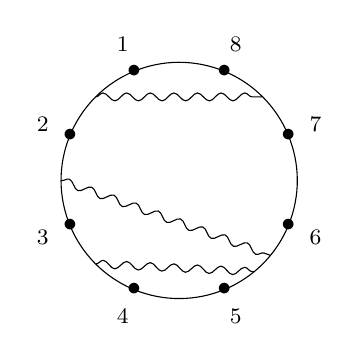
\begin{tikzpicture}[rotate=67.5,baseline=(current bounding box.east)]
	\begin{scope}
	\drawWLD{8}{1.5}
	\drawnumbers
	\drawprop{1}{0}{7}{0}
	\drawprop{3}{0}{5}{-1}
        \drawprop{2}{0}{5}{1}
		\end{scope}
	\end{tikzpicture}\eas and $W' = (\{(1,4), (3,5), (6,7), (8,1), (8,1)\}, [8])$ as \bas W'\ =\ 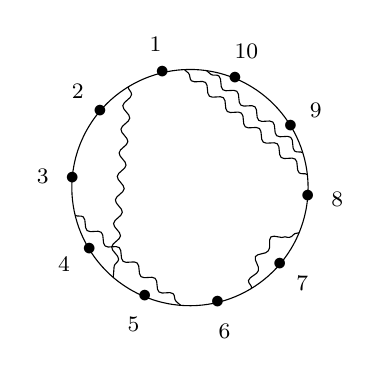
\begin{tikzpicture}[rotate=67.5,baseline=(current bounding box.east)]
	\begin{scope}
	\drawWLD{10}{1.5}
	\drawnumbers
	\drawprop{1}{0}{4}{0}
	\drawprop{3}{0}{5}{0}
        \drawpropbend{6}{0}{7}{0}{35}
	\drawprop{8}{1}{10}{-1}
 	\drawprop{8}{-2}{10}{2}
		\end{scope}
	\end{tikzpicture}\;.\eas 
Note that the pairs indicating the propagators are unorderer. That is if the propagator $p$ ends on the third and fifth edges, we may write $p = (3,5)$ or $p(5,3)$. In this paper, we use the convention that $p = (i, j)$, with $i$ preceeding $j$ in the natural linear order on $[n]$: $i < j$. Furthermore, we use the convention that if two propagators have endpoints on the same edge, they are drawn so that they do not cross. 

In the physics literature, we are only intersted in a certain subclass of these graphs, called admissible Wilson loop diagrams. An \emph{admissible} Wilson loop diagram, $W = (\cP, [n])$ satisfies the following conditions:
\begin{enumerate}
\item \textbf{Non-crossing} No pair of propagators $p, q \in \cP$ cross in the interior of $W$. That is, if $p = (i,j), \; q = (k, l) \in \cP$ written such that if $i < k$ then $l <j$. 
\item \textbf{Local Density} Any subset of propagators $ P \subset \cP$ is supported by at least 3 more vertices than the number of propagators in $P$: $|V_P| \geq |P| + 3$. 
\item \textbf{Global Density} There are at least 4 more vertices in the diagram than there are propagators. That is $n \geq |\cP| + 4$.
\end{enumerate} 

Note that the diagram $W$ above is admissible, while $W'$ is not. Furthermore, note that local density implies that one cannot have a propagators $p = (i, i+1)$ or pairs of propagators with the same endpoints: $p = q = (i, j)$.

For the remainder of this paper, we restrict our attention only to admissible Wilson loop diagrams.

In \cite{Wilsonloop} the authors show that each admissible Wilson loop diagram is assoicated to a positroid, $M(W)$, or a matroid that can be represented by a matroid, with a base set $[n]$. A subset $V \in [n]$ is not independent if and only if it contains a subset $U \subset V$ such that $|\Prop (U)| \leq |U|$ (thm \cite{??}). \todo{make result?} For instance, in $W$ above, the vertices $\{7,8\}$ are not independent since they only support one propagator between them. Therefore, no set of vertices containing $\{7, 8\}$ can be independent either. On the other hand, the vertices $\{3,4\}$ support two propagators, and thus are independent. The set $\{3,4, 5\}$ are three vertices supporting 2 propagators, and thus not independent. However, $\{2, 3, 4\}$ is a set of three vertices supporting 3 propagators, and is thus independent.

Furthermore, by virtue of the non-crossing restriction, the Wilson loop diagrams represent positroids (\cite[]). In other words, admissible Wilson loop diagrams can be represented by real valued matrices with all positive maximal minors.

\subsection{Matrices and positroids\label{sec:matrixdefs}}

Wilson loop diagrams have a natural matrix representation that bridges the combinatorics to geometric subspaces of the positive Grassmannians, which we discuss next.

For each propagator $p \subset \cP$ in admissible Wilson loop diagram, $W = (\cP, [n])$, associate a $4$ dimensional subspace of $\RP^{n+1}$ of the form \bas Y_p = \begin{cases}  c_{p,i} &  i = 0 \textrm{ or } i \in V_p \\ 0 &  \textrm{else,}\end{cases} \eas where $c_{p,i}$ are real valued variables. Then one may associated to $W$ a subspace of $\Grall(k, n+1)$ parametrized by the $Y_p$. That is, given the Wilson loop diagram $W$ above, with $p = (1,7)$, $q = (3,5)$ and $r = (2,5)$, one may write \bas C_*(W) = \begin{bmatrix} c_{p,0} & c_{p,1} & c_{p,2} & 0 &0 &0 &0 &c_{p,7} & c_{p,8} \\  c_{q,0} & 0 & 0 &c_{q,3} & c_{q,4} &  c_{q,5} & c_{q,6} & 0 & 0 \\ c_{r,0} & 0 & c_{r,2} & c_{r,3} & 0  &c_{r,5} & c_{r,6} & 0 &0\end{bmatrix}\eas

We define the matrix $C(W)$ to be the one defined by ignoring the first column of $C_*(W)$.  In the running example, \bas C(W) = \begin{bmatrix}  c_{p,1} & c_{p,2} & 0 &0 &0 &0 &c_{p,7} & c_{p,8} \\    0 & 0 &c_{q,3} & c_{q,4} &  c_{q,5} & c_{q,6} & 0 & 0 \\  0 & c_{r,2} & c_{r,3} & 0  &c_{r,5} & c_{r,6} & 0 &0\end{bmatrix}\eas

\begin{rmk}
Note that, as a subspace of $\Grall(k, n)$ (resp. $\Grall(k, n+1)$), or ordering of the rows in $C(W)$, resp. $C_*(W)$ do not matter.
\end{rmk}


The matroidal properties of Wilson loop diagrams derived in \cite{Wilsonloops}  can be verified by considering the independent columns of $C(W)$. Namely, 
\begin{enumerate} 
\item Theorem [???] of \cite{Wilsonloops} states that a set of vertices of a Wilson loop diagram, $(\cP, [n])$  is independent if and only if no subset supports fewer propagators than vertices in the subset. I.e. $V \subset [n]$ is independent if, for all $U \subseteq V$, $\Prop(U) \geq |U|$. In terms of rows and columns of $C(W)$, this simply states that any set of columns of $C(W)$ contains a dependent subset if said subset is non-zero on fewer rows than columns in the subset.
\item Theorem [???] shows that all admissible Wilson loop diagrams correspond to positroids. This means that, as matroids, the Wilson loop diagrams can be represented by matrices with all positive maximal minors. That is, the subspace of $\Grall(k,n)$ parametrized by $C(W)$ intersects $\Gr(k,n)$.
\end{enumerate}

Following the conventions of \cite{casestudy, generalcombinatorics1}, we call the positroid cell defined by the Wilson loop diagram $W$, $\Sigma(W)$. In \cite{basisshapeloci}, the author shows that the closure of the subspace of $\Gr(k,n)$ parametrized by the matrices $C(W)$ is $\overline{\Sigma(W)}$\sanote{I haven't defined what a positoid cell is}. Let $G(W)$ be the subspace of $\Gr(k,n)$ parametrized by $C(W)$. In other words, the space $G(W)$ differs from the positroid cell $\Sigma(W)$ only on a set of measure 0. For an explict example of where these spaces differ, see Example \ref{eg:closuresmatch}. The author of \cite{basisshapeloci} also shows each $\Sigma(W)$ is a $3k$ dimensional cell.

In \cite{non-orientable}, the authors show that  the subspace of $\Grall(k,n)$ parameterized by $C_*(W)$ can be viewed as a real $k$ bundle over the space parametrized by $C(W)$ . Restricting to $G(W)$ gives the vector bundle $G_*(W) \rightarrow G(W)$. As shown in Theorem [??] of loc. cit., the space $G_*(W)$ is not orientable. 

We have now constructed a map from Wilson loop diagrams to the positroid cells. Let $\cW_{k,n}$ be the set of all admissible Wilson loop diagrams with $k$ propagators and $n$ vertices. Then \ba \cW_{k,n} \leftrightarrow (\RP^4 )^{\times k} \hookrightarrow (\RP^{n+1} )^{\times k} \leftarrow G(W)  \;. \label{eq:maps}\ea The composition of the first two maps comes from the definition of the vectors $Y_p$.  The map $G_*(W) \rightarrow (\RP^{n+1} )^{\times k}$ is formed by setting the first entry of each $Y_p$ to 1. (Note, that in making this choice, we are deliberately preventing the variables in the first column of $C_*(W)$ from being $0$. However, this is okay as those values correspond to the physical poles of the scattering amplitude, and therefore are not the subject of this paper.) Under this choice, it is a dense inclusion for each $W \in \cW_{k,n}$. In particular, this map misses exactly the points in the image of $W$ in $(\RP^{n+1} )^{\times k}$ where the set of vectors $Y_p$ would not have full rank when evaluated. However, this is a space of measure $0$ in the image of $W$ in $(\RP^{n+1} )^{\times k}$. \sanote{haven't said anything about exact subdiagrams yet.}

\subsection{Integrals and poles \label{sec:integrals}}

The Wilson loop diagrams represent the tree level contributions to the scattering amplitudes in the physical theory N=4 SYM. The holomorphic Wilson loop for $n$ particles and $k$ propagators gives the contribution to the n particle scattering amplitude of N=4 SYM by $k$ propagators. The tree level contribution to this amplitude is given by a sum of integrals associated to admissible Wilson loop diagrams: \ba \cA_{k,n}^{tree} = \sum_{W \subset \cW_{k,n}} I(W) \;.\label{eq:treelevelamplitude}\ea The scattering amplitude is a functional on the particles of the theory, represented in twistor space. In this case, the external data are represented as $n$ sections of a $k$ dimensional real vector bundle over a real twistor space, $\{Z_1, \ldots, Z_n\}$  such that the $n \times n+4$ matrix who's $i^{th}$ row is $Z_i$ has positive maximal minors. Furthemore, we fix a guage section, $Z_0$, which can be taken, without loss of generality to be a $0$ section. We define the matrices \bas \cZ = \begin{bmatrix} - & Z_1& - \\ & \vdots &  \\ - & Z_n& -\end{bmatrix} \; ; \; \cZ_* = \begin{bmatrix}- & Z_0& - \\  - & Z_1& - \\ & \vdots & \\  - & Z_n& -\end{bmatrix} \; .\eas By the above, $\cZ$ has positive maximal minors. 

We are now ready to define the integrals assoicated to each Wilson loop diagram $W = (\cP, [n])$, with $k = |\cP|$:

\begin{dfn} \label{dfn:I(W)} \bas \cI(W) (\cZ_*)  = \int_{(\RP^4)^k} \frac{\prod_{p \in \cP} \prod_{v \in V_p} dc_{p, v}}{R(W)} \delta^{4k|4k}(C_*(W) \cdot \cZ_*) \eas where, for $X$ a $k \times n+4$ matrix, \bas \delta^{4k|4k}(X) = \prod_{b =1}^k (X_{b, 4+b})^4\delta^4((X_{b,1},X_{b,2},X_{b,3},X_{b,4}))  \eas and $R(W)$ is a polynomial determined from the $W$ as follows: 
\begin{enumerate}
\item For each edge $e \in [n]$, let $\{q_1, \ldots, q_s \}$ be the propagators incident on the edge $e$, ordered according to their proximity to vertex $e$. 
\item Define $R_e = c_{q_1, e+1} \big(\prod_{r = 1}^{s-1} (c_{q_r, e}c_{q_{r+1}, e+1} - c_{q_r, e+1}c_{q_{r+1}, e})\big) c_{q_s, e}$
\item $R(W) = \prod_{e \in [n]} R_e$
\end{enumerate} \end{dfn}

Note that in this definition, we take the integral over $(\RP^4)^k$, while previously, we have referred to the matrices as parametrizing subspaces of $\Gr(k,n)$. This is permissible due to the density arguments following display \eqref{eq:maps}.

\begin{dfn}
We say that $q_i$ and $q_{i+1}$ are adjascent on the edge $e$.
\end{dfn}

In \cite{generalcombinatoricsII}, we show that $R(W)$ is exactly the product of the prime factors of the determinants of $C(W)$ defined by the Grassmann necklace of $M(W)$. In combination with the results of \cite{basisshapeloci}, we show that 

\begin{prop}
All the factors of $R(W)$ vanish on the boundary of $\Sigma(W)$.
\end{prop}


\begin{proof}
Let $\{I_1, I_2, \dots, I_k\}$ be the Grassmann necklace associated $\Sigma(W)$. From Proposition 5.3 in \cite{generalcombinatoricsII},
%
\begin{displaymath}
R(W) = \mathrm{rad}\left(\prod_{i = 1}^{k} \Delta_{I_i}\right).
\end{displaymath}
%
From Theorem 5.15 in \cite{knutsonlamspeyerjuggling}, the ideal of functions defining the variety $\overline{\Sigma(W)}$ is generated by $\{\Delta_I : I \notin M(W)\}$. From (THEOREM NUMBER) in \cite{basisshapeloci}, $G(W) \subset \overline{\Sigma(W)}$ and hence ever function vanishing on $\Sigma(W)$ vanishes on $G(W)$. Theorem 5.1 in \cite{knutsonlamspeyerjuggling} implies that the open positroid variety $\Sigma(W)$ is defined as a subset of $\overline{\Sigma(W)}$ by
%
\begin{displaymath}
\Delta_{I_1}, \Delta_{I_2}, \dots, \Delta_{I_k} \neq 0.
\end{displaymath}
%
Thus, the subset of $G(W)$ where $R(W)$ vanishes is exactly
%
\begin{displaymath}
G(W) \setminus \Sigma(W) \subset \overline{\Sigma(W)} \setminus \Sigma(W). \qedhere
\end{displaymath}
\end{proof}

\begin{eg} \label{eg:closuresmatch}
This example illustrates the differences between the sets $G(W)$, $\Sigma(W)$, and $\overline{\Sigma(W)}$. Let
\bas C(W) =
\begin{bmatrix}
c_{p,1} & c_{p,2} & 0 &c_{p,4} & c_{p,5} & 0 \\
c_{q,1} & c_{q,2} & 0 & 0 & c_{q,5} & c_{q,6}
\end{bmatrix}.\eas
\noindent
Let $\Sigma(W)$ and $\overline{\Sigma(W)}$ be the associated open and closed positroid cells respectively.

The point represented by
\begin{displaymath}
\begin{bmatrix}
1 & 1 & 0 & 1 & 1 & 0 \\
1 & 1 & 0 & 0 & 1 & 1
\end{bmatrix}
\end{displaymath}
\noindent
is in $G(W) \setminus \Sigma(W)$, since the minor $\Delta_{I_1} = \Delta_{12}$ vanishes. Hence,
%
\begin{displaymath}
R(W) = (c_{p,1}c_{q,2} - c_{p,2}c_{q,1}) c_{p,1} c_{p,4} c_{p,5} c_{q,2} c_{q,5} c_{q,6}
\end{displaymath}
\noindent
vanishes at this point.

The point represented by
\begin{displaymath}
\begin{bmatrix}
1 & 0 & 0 & 1 & 0 & 1 \\
0 & 1 & 0 & 1 & 1 & 1
\end{bmatrix}
\end{displaymath}
\noindent
is in $\Sigma(W) \setminus G(W)$ since there is no point in $G(W)$ where $\Delta_{45},\Delta_{56} \neq 0$ and $\Delta_{46} = 0$.

The point represented by
\begin{displaymath}
\begin{bmatrix}
0 & 0 & 0 & 0 & 1 & 0 \\
0 & 0 & 0 & 0 & 0 & 1
\end{bmatrix}
\end{displaymath}
\noindent
is in $\overline{\Sigma(W)} \setminus \Sigma(W) \cup G(W)$.
\end{eg}

This fact has been shown explicitly in the case of $n = 6$ and $k=2$, however, has not been shown in general.

It is worth noting here that with the $N^kMHV$ (tree level) amplitude
on $n$ points is taken to be the sum of all the integrals associated
to Wilson loop diagrams. Above, we have shown that the spurious poles
all fall on the boundaries of the geometric space. Below, we show that
all the spurious poles do, in fact, cancel. However, unlike in the
Amplituhedron story, one cannot assoiciate a geometric meaning to the
sum of these integrals. In \cite{non-orientable}, the authors show
that while the subspace of $\Grall (k,n+1)$ associated to each
$C_*(W)$ is orientable, the union of said spaces are not. Therefore,
one cannot interpret the sum of the associated integrals as the volume
of a geometric space. This result has also been shown explicitly and
separately in \cite{Heslop-Stewart} which calucates contradiction that
occures if one attempts this interpretation.

Here, we propose a different geometric interpretation of the sum of
these integrals. One can consider \hlfix{$G_*(W)$ as a $k$-dimensional
  line bundle over $G(W)$ }{Is this true, or is this only true on
  $\Sigma(W)$?} \cite{non-orientable}. Then, we may consider the
cancelation of spurious poles on any section of the bundle. In fact,
for the spurious poles, one typically sets the values of $c_{p,0}$ to
be $\pm 1$, as the physical poles of $N=4 SYM$ occur when $c_{p,0} =
0$. \hlfix{After fixing any such section, the sum can be interpreted as a
volume on this section.}{verify that this is consistent with \eqref{eq:maps}}
{\color{red} Do we have a proof that the space parametrized by the $C_*(W)$, or tiled by the $\Sigma(W)$, is orientable? Can we create such a proof using arguments similar to that showing that the full space is non-orientable? maybe skip the volume argument in this paragraph altogether?}

\section{The poles of Wilson loop diagrams}

\subsection{Cluster algebras, frozen variables, Grassmann Necklaces}

As a brief aside, we note that the polynomial $R(W)$ has appeared in relation to a cluster algebra associated to the positroid $\Sigma(W)$. Let $\mathcal{I} = \{I_1,I_2, \dots, I_k\}$ be the Grassmann necklace associated to $\Sigma(W)$. So, $I_j$ is that minimal set in the $j^{th}$ cyclic shift of the Gale order on sets such that the Pl\"ucker coordinate $\Delta_{I_j}$ is non-vanishing on $\Sigma(W)$. Let $\mathcal{I}^{\ast} = \{I^{\ast}_1, I^{\ast}_2, \dots, I^{\ast}_{k}\}$ be the reverse Grassmann necklace associated to $\Sigma(W)$. That is, $I^{\ast}_j$ is that maximal set in the $j^{th}$ cyclic shift of the Gale order on sets such that the Pl\"ucker coordinate $\Delta_{I^*_j}$ is non-vanishing on $\Sigma(W)$. Following Chapter 5 of \cite{knutsonlamspeyerjuggling} replacing Schubert varieties in the Grassmannian with reverse Schubert varieties, one sees $\Sigma(W)$ can equivalently be defined as an intersection of reverse Schubert varieties. Running the combinatorial algorithm for {\color{red} citation?} produces a Grassmann necklace for $\Sigma(W)$ given the diagram $W$ in clockwise, rather than counter clockwise, order yields the reverse Grassmann necklace for $\Sigma(W)$. Define
%
\begin{displaymath}
R^{\ast}(W) = \mathrm{rad}\left(\prod_{i = 1}^{k} \Delta_{I^{\ast}_i}\right).
\end{displaymath}

%{\color{red} the paragraph above might have been kind of fast, but i think it gives enough to convince the reader of the following lemma we had been including? at least enough for an aside section?

%\begin{lem}
%We can read the backwards GN off the diagram by reversing direction. 
%\end{lem}}


\begin{thm}
Using the notation from above, $R^{\ast}(W) = R(W)$.
\end{thm}

\begin{proof}
This follows from the fact that $R^{\ast}(W)$ and by $R(W)$ are both radical polynomials defining the same subvariety of the Wilson loop cell $G(W)$. 

From Section 5 of \cite{knutsonlamspeyerjuggling}, the open positroid variety $\Sigma(W)$ is defined as a subset of $\overline{\Sigma(W)}$ by $\Delta_I \neq 0$ for all $I \in \mathcal{I}$, where $\mathcal{I}$ is the Grassmann Necklace of $\Sigma(W)$. So, $\prod_{I \in \mathcal{I}} \Delta_I$ defines the subvariety $(\overline{\Sigma(W)} \setminus \Sigma(W)) \subset \overline{\Sigma(W)}$, the boundary of the open positroid inside the closed positroid. 

Let $G(W)$ be the geometric space parameterized by the Wilson Loop diagram $W$. From Theorem ?? in \cite{basisshapeloc}, $G(W) \subset \overline{\Sigma(W)}$. Let $V$ be the subset of $G(W)$ which is the pull back of the set in $(\mathbb{RP}^{4})^{k}$ where $R(W)$ vanishes via (\ref{eq:maps}). Then,

%
\begin{equation} \label{eqn:rw_vanishes}
\begin{split}
V & = V \cap \overline{\Sigma(W)} \\
& = G(W) \cap (\{\Delta_I = 0 : \exists I \in \mathcal{I}\} \cap \overline{\Sigma(W)}) \\
& = G(W) \cap (\overline{\Sigma(W)} \setminus \Sigma(W)) \\
& = G(W) \setminus \Sigma(W).
\end{split}
\end{equation}

Theorem ?? from \cite{generalcombinatorics2} shows that $R(W)$ generates the radical of the ideal generated by $\prod_\mathcal{I} \Delta_{I_i}$.

Following Section 5 of \cite{knutsonlamspeyerjuggling} replacing Schubert varieties with opposite Schubert varieties, $\Sigma(W)$ is similarly defined as a subset of $\overline{\Sigma(W)}$ by $\Delta_{I^{\ast}} \neq 0$ for all $I^{\ast} \in \mathcal{I}^{\ast}$. So, $\prod_{I^{\ast} \in \mathcal{I}^{\ast}} \Delta_{I^{\ast}}$ also defines the subvariety $(\overline{\Sigma(W)} \setminus \Sigma(W)) \subset \overline{\Sigma(W)}$. Following (\ref{eqn:rw_vanishes}), the pull back of the vanishing set of $R^{\ast}(W)$ from $(\mathbb{RP}^4)^{k}$ to $\Grall(k,n)$ is also $G(W) \setminus \Sigma(W)$. Pulling this set back to $(\mathbb{RP}^4)^{k}$, polynomials $R(W)$ and $R^{\ast}(W)$ vanish on the same set. $R^{\ast}(W)$ is radical by definition. Since $R^{\ast}(W)$ and $R(W)$ are radical polynomials defining the same variety, $R^{\ast}(W) = R(W)$.
\end{proof}


\begin{rmk}
Be careful that above $R(W)$ and $R^{\ast}(W)$ are both polynomials in the matrix entries $c_{p,i}$. The radicals taken are over the polynomial ring in these variables, defining a variety in the space of $n \times k$ matrices. To pass to the Grassmannian and obtain the variety $\overline{\Sigma(W)}$, one must further remove singular matrices and quotient by the left action of $\mathrm{Gl}(k)$. 
\end{rmk}

{\color{red} finally, have a paragraph just saying what role $R^{\ast}(W)$ plays in the cluster algebra stuff (at least as well as i understand it)}

%\begin{thm}
%If a WLD does not have a non-trivial exact subdiagram, then $C(W)$ is its unique  minimal representation. {\color{red} Again, do we need this?...i don't think we need this for this section?}
%\end{thm}

\subsection{Geometry of the poles}

Note that not every co-dimension one boundary of a $\Sigma(W)$ contains a factor of $R(W)$. In order to reach a boundary of a positroid cell, one must send certain minors to 0 while not causing any perviously vanishing minors to become positive. Sending parameters to $0$, which causes the polynomial $R(W)$ to vanish, is certainly one way to do this. However, the boundary of $\Sigma(W)$ contains other positroid cells which do not necessarily intersect the vanishing set of $R(W)$. For instance, consider the following example:

\begin{eg}
The Wilson loop diagram\bas V_1 =  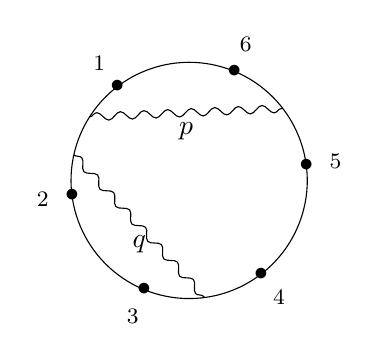
\begin{tikzpicture}[rotate=67.5,baseline=(current bounding box.east)] \begin{scope}
	\drawWLD{6}{1.5}
	\drawnumbers
	\drawlabeledprop{1}{-1}{5}{0}{$p$}
	\drawlabeledprop{1}{1}{3}{0}{$q$}
	\end{scope} \end{tikzpicture} \eas Has a matrix \bas C(V_1) = \begin{bmatrix} c_{p,1} &  c_{p,2} & 0 & 0 &c_{p,5} &c_{p,6} \\c_{q,1} &  c_{q,2} & c_{q,3} &  c_{q,4}& 0 & 0 \end{bmatrix}\; . \eas From \cite{casestudy}, we see that this shares a boundary with the positroid cells parametrized by \bas C(N_2) = \begin{bmatrix} *&  * & 0& 0 &0 &* \\ 0 &  * & *&  *& * & * \end{bmatrix}\eas and \bas C(N_3) = \begin{bmatrix} *&  * & *& 0 &0 &0 \\0 &  * & *&  *& * & * \end{bmatrix} \;. \eas Here the $*$ correspond not no-zero, independent real variables. In particular, the common boundary is parametrized by the matrix \bas \begin{bmatrix} *&  * & 0& 0 &0 &0 \\0  &  * & *&  *& * & * \end{bmatrix}.\eas
This common boundary is 5 dimensional, parameterized for instance by setting one of the stars in each row to be 1 and allowing the other entries to be free. From (\ref{eqn:rw_vanishes}), the vanishing set of $R(V_1)$ is exactly $G(V_1) \setminus \Sigma(V_1)$, where $G(V_1)$ is the geometric space parameterized by $V_1$. On the boundary (open) positroid cell, $\Delta_{13}$ and $\Delta_{15}$ are both non-vanising. On $G(V_1)$, the nonvanishing of $\Delta_{13}$ and $\Delta_{15}$ implies the nonvanishing of $\Delta_{35}$. Since $\Delta_{35}$ vanishes on the boundary positroid cell in question, $G(V_1)$ does not intersect this boundary and hence $R(V_1)$ does not vanish.
\end{eg}

For the following proposition, we extend the definitions of $\Prop(V)$ and $V(p)$ for general variable valued matrices and not just those representing Wilson loop diagrams.

\begin{dfn}
Let $C$ be a variable valued matrix. Denote by $r$ a row of $C$, and $c$ a column of $C$. Then we write $\Cols(r)$ to be the columns where the row $r$ has non-zero entries. Similarly, write $\Rows(c)$ to be the rows where the column $c$ has non-zero entries. 
\end{dfn}

Note that if $C = C(W)$ the matrix associated to a Wilson loop diagram, the rows are the propagators and the columns are the vertices. Then $\Rows(c) = \Prop(c)$ and $\Cols(r) = V(r)$.

\begin{prop}
Let $\Sigma$ be a positroid cell of dimension $d$ in $\Gr(k,n)$, and $C$ be a variable valued matrix realizing $\Sigma$ with $d + k$ independent variables, and $M(C)$ the associated matroid. Let $V$ and $W$ be \hlfix{cyclic flats}{needs definition} of less than full rank ($\rk (V), \; \rk(W) <k$) such that one is not contained in the other ($W \subsetneq V$) and that $M(C)$ cannot be decomposed into disconnected matroids with $V$ or $W$ contained in one of the summands. Without loss of generality, suppose that $|\Rows(V) \setminus \Rows(W)| \geq |\Rows(W) \setminus \Rows(V)|$. A matroid defined by:
\begin{itemize}
\item Taking the entries of $C|_{W}$ and moving them to a 0 entry in $\Rows(V)$ and $\Cols(V\cup W)$. \todo{(note, I don't think the colums need to be respected)} 
\item then zeroing out the original elements in $C|_{W}$.
\end{itemize}
Replacing the cyclic flats $W$ and $V$ with $W \cup V$ reduces the dimension of the positroid cell thus defined.
\end{prop}

\begin{proof} First we observe that if the bases set of one positroid cell, $\Sigma'$ is contained in the bases set of another, $\Sigma$, then $\Sigma'$ is on the boundary of $\Sigma$. Let $C'$ be the matrix formed from $C$ by the algorithm above. Let $\Sigma'$ be the positroid cell defined by the Grassmann Necklace of $M(C')$. We show that $\Sigma'$ is on the boundary of $\Sigma$. 

To do this, we compare the Grassmann necklaces of $M(C)$ and $M(C')$. Call these $GN(C)$ and $GN(C')$ respectively, as they can be read off directly from the matrices. In particular, we note that $GN(C) \neq GN(C')$. To see this, first note that $\rk(V)$ (resp. $\rk W) >0$. If this were not true, then whichever flat had rank $0$ would be contained in the other flat, which contradicts our hypothesis. Then we note that some vertex of $V$ (resp. $W$)  appears at least once in $GN(C)$. To see this, note that any element that does not ever appear in $GN(C)$ has rank $0$. Since neither $V$ nor $W$ has rank $0$, they must each contain at least one element that appears in $GN(C)$. Therefore, we know that there exists some $I_j \in GN(C)$ such that $I_j \cap W \neq \emptyset$. Fix such a $j$ and let $a \in  I_j \cap W$ be an element of $W$ that is in said $I_j$. Let $I'_j$ be the correposponding element of $GN(C')$. We claim that $I_j \neq I_j'$. That is, the $j^{th}$ minor in $GN(C')$ is not the same as the $j^{th}$ minor of $GN(C)$. This shows that $M(C)$ and $M(C')$ define two different positroid cells. Then it remains to show that the the basis set $\cB$ of $M(C)$ contains the basis set $\cB'$ of $M(C')$. 

\emph{Proof of claim:}Suppose, for contractiction, $I_j = I'_j$. Write $I_j = v_1 \ldots v_k$ with $v_i <_j v_{i+1}$. By definition fo the Grassmann Necklace, $a$ is the first column in the $>_j$ ordering of the columns of $C$ that is not contained in the flat defined by previous elements of $I_j$: $\textrm{cl}(\{v_i | v_i <_j a \})$ in $M(C)$. In $C'$, the non-zero entries in the column $a$ lie in the rows where $V$ has non-zero entries: $\Cols(a) \subset \Cols(V)$. Since $a \in I'_j$, the flat $V \cup W$ in $M(C')$ is not contained in the the flat defined by the previous elements of $I'_j$: $V \cup W \not \subset \textrm{cl}(\{v_i | v_i <_j a )$ in $M(C')$. Since $\Rows(V \cup W)$ in $C'$ is the same as $\Rows(V)$ in $C$, the flat defined by $V$ in $M(C)$ is is not contained in the the flat defined by the previous elements of $I_j$: $V\not \subset \textrm{cl}(\{v_i | v_i <_j a ) \}$ in $M(C)$. \todo{is $U$ uniquely defined?} Let $U \subset I_j$ be the smallest subset of $I_j$ that is needed to ensure that $V \subset \textrm{cl}(\{v_i | v_i <_j a \} \cup U)$ in $M(C)$. Note that $a$ preceeds all elements of $U$, by construction s $a \leq_j u$ for all $u \in U$ in $M(C)$. However, also by construction, $a \in U$ in $M(C')$. Therefore, there must be some $b \in U$ that is in $M(C)$ but not in $M(C')$, thus violating $I_j = I'_j$.
 
To see that basis set $\cB$ of $M(C)$ contains the basis set $\cB'$ of $M(C')$, note that any $B \in \cB$ that that does not intersect $V \cup W$ is also a basis set of $\cB'$ and vice versa. Any basis set $B \in \cB$ intersecting $W$ is not a basis set in $\cB'$. Let $B' \in \cB'$ be a basis set of $M(C')$ intersecting $V\cap W$. Partition $B'$ into two sets, those elements in $V \cup W$  and those not: $B' = B'_1 \cup B'_2$ with $B'_1 \subset V \cup W$ and $B'_2 \cap (V \cup W) = \emptyset$. If $B'$ were not a basis set of $M(C)$ ($B' \not \in \cB$), then $\Rows(V) \cap \Rows(B'_2) = \emptyset$ and $\Rows(W) \subset \Rows(B'_2)$ in $M(C)$. But this contradicts the deomposability hypothesis.
\end{proof}


\begin{thm}
Let $W$ be an admissible Wilson loop diagram and let $G' \subset G(W)$ be the vanishing locus of a single factor of $R(W)$ inside $G(W)$ and suppose that $G'$ has codimension $1$ in $G(W)$. Let the open positroid $\Sigma'$ be the boundary of $\Sigma(W)$ corresponding to $G'$. Then, $G'$ is dense in $\Sigma'$.
\end{thm}

\begin{proof}
\begin{itemize}
\item Entry vanishing, cite basis shape paper.
\item $2 \time 2$ factor vanishing, see notes. The subtle thing here is that the hard part is normally showing that the dimension is correct in this case, but here I built it into the hypothesis (which is kinda lame, but I think captures the situation we're in).
\end{itemize}
\end{proof}

\begin{thm}
All the codimension 1 poles of admissible Wilson loop diagrams cancel.
\end{thm}

\begin{proof}
By construction, the primitive factors of $R(W)$ either correspond to $1 \times 1$ or $2 \times 2$ minors of $C(W)$. Infact, by construction, setting a $1 \times 1$ minor to zero corresponds to, in the notaton of definition \ref{dfn:I(W)}, setting $c_{q_1, e+1} = 0$ or $c_{q_s, e} = 0$. We depict this diagramatically as (for $e = 8$) \bas   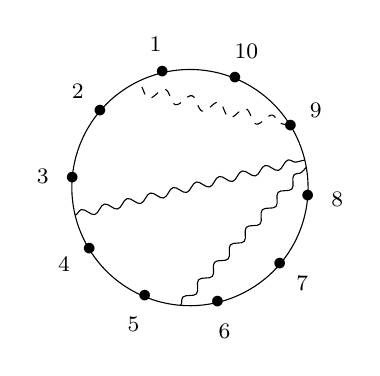
\begin{tikzpicture}[rotate=67.5,baseline=(current bounding box.east)]
	\begin{scope}
	\drawWLD{10}{1.5}
	\drawnumbers
	\boundaryprop{1}{0}{9}{propagator, dashed}
	\drawprop{3}{0}{8}{0}
        \drawprop{5}{0}{8}{-1}
		\end{scope}
	\end{tikzpicture} \text{ or } 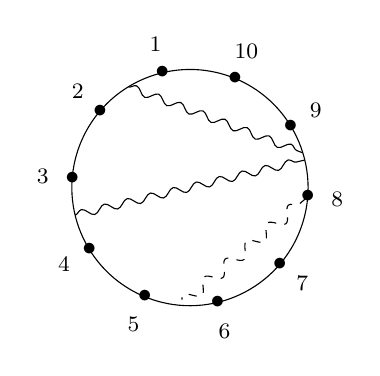
\begin{tikzpicture}[rotate=67.5,baseline=(current bounding box.east)]
	\begin{scope}
	\drawWLD{10}{1.5}
	\drawnumbers
	\drawprop{1}{0}{8}{1}
	\drawprop{3}{0}{8}{0}
        \boundaryprop{5}{0}{8}{propagator, dashed}
		\end{scope}
	\end{tikzpicture} \;.\eas That is, a setting a $1\times 1$ minor to zero can be depicted by supporting a single propagator on the remaining three vertices. Similarly, the $2 \times 2$ minors correspond to setting two of the variables supporting adjasacent propagators as scalar multiples of each other. In the same example, we draw this as \bas   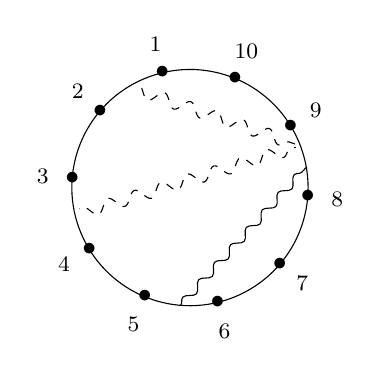
\begin{tikzpicture}[rotate=67.5,baseline=(current bounding box.east)]
	\begin{scope}
	\drawWLD{10}{1.5}
	\drawnumbers
	\modifiedprop{1}{0}{8}{2}{propagator, dashed}
	\modifiedprop{3}{0}{8}{2}{propagator, dashed}
        \drawprop{5}{0}{8}{-1}
		\end{scope}
	\end{tikzpicture} \;, \eas or setting a $2 \times 2$ minor is depicted by making two adjascent propagators meet on the common edge.

We first consider all the possible degree 1 factors of $R(W)$. Write $W = (\cP, [n])$ with $p= (i,j)  \in \cP$. Suppose $j > i+2$ (i.e. if $V(p)$ does not consist of $4$ cyclically consecutive vertices) and, wihtout loss of generality, assume $c_{p, i}$ is a factor of $R(W)$. Then if $q = (i+1, j) \not \in \cP$ the we may define another diagram $W' = ((\cP \setminus p) \cup q, [n])$ such that $\lim_{c_{p, i} \rightarrow 0} I(W) = -\lim_{c_{q, i+2} \rightarrow 0} I(W')$, where the negative sign comes from the evaluation of $\delta^{4k|4k}$ (see Lemma \ref{lem:movingpropnegative}). For more details on the minus signs, see \cite{casestudy, HeslopSteward, correlahedron}. By the arguments of \cite{basisshapeloci}, we see that this parametrizes a co-dimension 1 boundary of $\Sigma(W)$. It is easy to check that $W'$ sasisfies both non-crossing (because $W$ satisfies non-crossing) and the density (because $q \not in \cP$, and $W$ satisfies density) conditions for admissibility. Thereofre $W'$ is admissible. 

If $q \in \cP$, then, the two rows of $\lim_{c_{p, i} \rightarrow 0}C(W)$ defined by the propagators $p$ (now supported on 3 vertices) and $q$ have non-zero entries in only 4 columns. Therefore, by the arguments of \cite{basisshapeloci}, we see that this parametrizes a co-dimension 2 boundary of $\Sigma(W)$. Therefore, we do not consider these poles. 

It remains to consider the degree one factors of $R(W)$ contributed by propagators of the form $p = (i, i+2)$. If $c_{p, i+1}$ or $c_{p, i+2}$ are factors of $R(W)$, then consider the propatators $q = (i-1, i+2)$ or $q = (i, i+3)$ respectively. If $q \not \in W$, then the diagram $W' = ((\cP \setminus p)\cup q, [n])$ is admissible, and the argument proceeds as above. If $c_{p, i}$ or $c_{p, i+3}$ are factors of $R(W)$, let $q = (i+1, i+3)$ or $q = (i-1, i+1)$ respectively. By the non-crossing condition, $p$ and $q$ cannot simultaneously exist in $W$. If $W$ does not contain another propagator of the form $(i+2, k)$ or $(i, k)$ respectfully, we may define an admissible diagram $W' = ((\cP \setminus p)\cup q, [n])$ (otherwise, $q$ would cross the existing propagator $(i+2, k)$ or $(i, k)$).  In this case, $\lim_{c_{p, i} \rightarrow 0} I(W) = -\lim_{c_{q, i+4} \rightarrow 0} I(W')$ where the negative sign comes from the same arguments as above. 

It remains to check the case when $c_{p, i}$ (resp. $c_{p, i+3}$) is a factor of $R(W)$ and there exists a propagator $(i+2, k)$ (resp. $(i, k)$) in $W$. In this case, the simple pole formed by taking the limit as $c_{p, i}$ (resp. $c_{p, i+3}$) goes to zero cancels with a pole coming from degree 2 factors contributed by other diagrams. Therefore, we return to this during the discussion of $2 \times 2$ minors. 

Next, we consider the degree 2 factors of $R(W)$. In order for such a factor to exist, there must be some edge of $W$, call it $i$, that has at least two propagators ending on it, say $p = (i, j)$ and $q = (i, k)$. Suppose $k > j+1$, that is, the other endpoints of $p$ and $q$ are not on adjascent edges. If $r = (j,k) \not \in \cP$, consider two other diagrams $W' = ((\cP \setminus p) \cup r, [n])$ and $W'' = ((\cP \setminus q) \cup r, [n])$. Since $k> j+1$ and $r \not \in \cP$, both $W'$ and $W''$ both satisfy density. Furthermore, since $W$ is admssible, and $p$ and $q$ are adjascent on the edge $i$, there does not exist a propagator $(i, m)$ with $j < m <k$, that is, that has one endpoint on the $i^{th}$ edge, and the other between the endpoints of $p$ and $q$. Therefore, $W'$ and $W''$ satisfy non-crossing. I.e, they are both admissible. \todo{still need a proof that this is a codimension 1 boundary.} We see from Lemma \ref{lem:Vdiagcancel} that after appropriate changes of parametrizations, one may write \bas \lim_{(c_{r,k}c_{q,k+1} -c_{r,k+1}c_{q,k})\rightarrow 0}I(W') +  \lim_{(c_{p,i}c_{q,i+1} -c_{p,i+1}c_{q,i})\rightarrow 0} I(W) + \lim_{(c_{p,j}c_{r,j+1} -c_{p,j+1}c_{r,j})\rightarrow 0}I(W'') = 0 \; .\eas That is, the limits represented by the following diagrams, paramterize the same codimension 1 subspace in the intersection $\Sigma(W) \cap \Sigma(W') \cap \Sigma(W'')$.  {\color{red} up to some density argument, right?} \bas 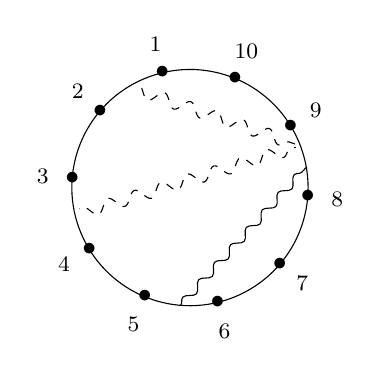
\begin{tikzpicture}[rotate=67.5,baseline=(current bounding box.east)]
	\begin{scope}
	\drawWLD{10}{1.5}
	\drawnumbers
	\modifiedprop{1}{0}{8}{2}{propagator, dashed}
	\modifiedprop{3}{0}{8}{2}{propagator, dashed}
        \drawprop{5}{0}{8}{-1}
		\end{scope}
	\end{tikzpicture} \leftrightarrow 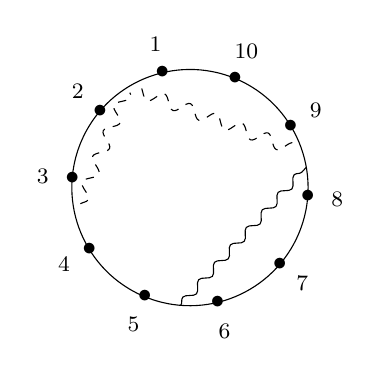
\begin{tikzpicture}[rotate=67.5,baseline=(current bounding box.east)]
	\begin{scope}
	\drawWLD{10}{1.5}
	\drawnumbers
	\modifiedprop{1}{0}{8}{1}{propagator, dashed}
	\modifiedprop{1}{0}{3}{0}{propagator, dashed}
        \drawprop{5}{0}{8}{-1}
		\end{scope}
	\end{tikzpicture} \leftrightarrow 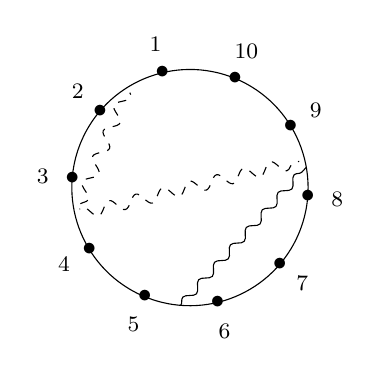
\begin{tikzpicture}[rotate=67.5,baseline=(current bounding box.east)]
	\begin{scope}
	\drawWLD{10}{1.5}
	\drawnumbers
	\modifiedprop{1}{0}{3}{0}{propagator, dashed}
	\modifiedprop{3}{0}{8}{0}{propagator, dashed}
        \drawprop{5}{0}{8}{-1}
		\end{scope}
	\end{tikzpicture}\eas In otherwords, these three codimension 1 boundaries cancel in the sum of integrals tha make up the amplitude.

If $k > j+1$ but the propagator $r =  (j,k) \in \cP$, then setting any of the minors $(c_{p,i}c_{q,i+1} -c_{p,i+1}c_{q,i})$, $(c_{p,j}c_{r,j+1} -c_{p,j+1}c_{r,j})$ or $(c_{r,k}c_{q,k+1} -c_{r,k+1}c_{q,k})$ to zero creates a codimension 2 boundary. \todo{Needs proof.}

It remains to check the case where $k = j+1$, i.e. $W$ contains a pair of propagotors configured as below: \bas 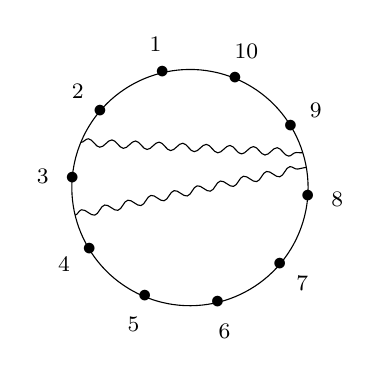
\begin{tikzpicture}[rotate=67.5,baseline=(current bounding box.east)]
	\begin{scope}
	\drawWLD{10}{1.5}
	\drawnumbers
	\drawprop{3}{0}{8}{-1}
	\drawprop{2}{0}{8}{1}
		\end{scope}
	\end{tikzpicture} \eas

Consider the diagrams $W' = ((\cP \setminus p) \cup r = (j, j+2), [n])$ and $W'' = ((\cP \setminus p) \cup s = (k-2, k), [n])$. Since the edge $r \not \in \cP$ (it would cross $q$ if it were), and $s \not \in \cP$ (it would cross $p$ if it were), we see that $W'$ and $W''$ satisfy both the non-crossing and density conditions, and thus are admissible. 

We see from Lemma \ref{lem:narrowVcancel} that pole defined by the limit of sending $(c_{p,i}c_{q,i+1} -c_{p,i+1}c_{q,i})$ to $0$ cancels with degree 1 poles in the diagrams in $W'$ and $W''$ under the correct parametrizations: \bas \lim_{(c_{p,i}c_{q,i+1} -c_{p,i+1}c_{q,i}) \rightarrow 0}I(W) + \lim_{c_{r, k-2}\rightarrow 0}I(W') + \lim_{c_{s, j+3}\rightarrow 0}I(W'') =0 \;.\eas That is, the limits represented by the following diagrams, paramterize the same codimension 1 subspace in the intersection $\Sigma(W) \cap \Sigma(W') \cap \Sigma(W'')$. \bas 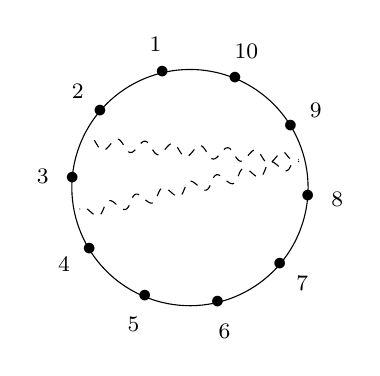
\begin{tikzpicture}[rotate=67.5,baseline=(current bounding box.east)]
	\begin{scope}
	\drawWLD{10}{1.5}
	\drawnumbers
        \modifiedprop{3}{0}{8}{0}{propagator, dashed}
	\modifiedprop{2}{0}{8}{0}{propagator, dashed}
	\end{scope}
	\end{tikzpicture} \leftrightarrow 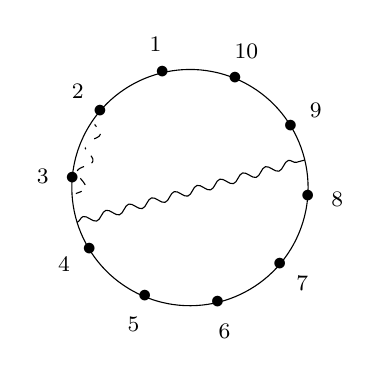
\begin{tikzpicture}[rotate=67.5,baseline=(current bounding box.east)]
	\begin{scope}
	\drawWLD{10}{1.5}
	\drawnumbers
        \drawprop{3}{1}{8}{0}
	\boundaryprop{3}{-1}{2}{propagator, dashed}
	\end{scope}
	\end{tikzpicture} \leftrightarrow 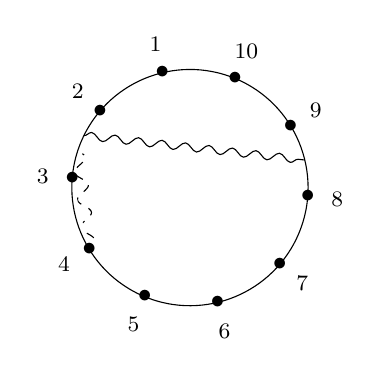
\begin{tikzpicture}[rotate=67.5,baseline=(current bounding box.east)]
	\begin{scope}
	\drawWLD{10}{1.5}
	\drawnumbers
        \drawprop{2}{-1}{8}{0}
	\boundaryprop{2}{1}{4}{propagator, dashed}
	\end{scope}
	\end{tikzpicture}\eas

Note that the degree one terms of $R(W)$ involved in this calculation are exactly the degree one factors whose cancelation was put off until discussion of the degree two terms.
\end{proof}

{\color{red} Worth noting that this can only be done on a section of the $\Gr(k,n)$ in the $\Grall(k, n+1)$ bundle (i.e. when whe consider $C(W)$ as the fundamental objects, and not $C_*(W)$. \cite{HeslopStewart, non-orientability} show that we cannot do this for the space in genral because of orientation issues.} 

\begin{appendices} 
\section{Graveyard of Technical Lemmas}
In this section, we present some calculations to aid in the understanding of the cancelation of spurious poles. Many of the results here can be found in \cite{casestudy, correlahedron, HeslopStewart}. However, they are presented here for completeness.

Recall from definition \ref{dfn:I(W)} that \bas \cI(W) (\cZ_*)  = \int_{(\RP^4)^k} \frac{\prod_{p \in \cP} \prod_{v \in V_p} dc_{p, v}}{R(W)} \delta^{4k|4k}(C_*(W) \cdot \cZ_*) \eas where, for $X$ a $k \times n+4$ matrix, \bas \delta^{4k|4k}(X) = \prod_{b =1}^k (X_{b, 4+b})^4\delta^4((X_{b,1},X_{b,2},X_{b,3},X_{b,4}))  \;.\eas Write $\cZ_*^i$ to indicate the $i^{th}$ column of $\cZ_*$ and $\cZ_*^\mu$ to indicate the matrix formed by taking the first 4 columns of $\cZ_*$. Then evaluating the integral $I(W)$ corresponds to localizing the expression \bas \frac{\prod_{b = 1}^k (Y_b \cdot \cZ_*^b)^4}{R(W)}\eas at the solution to $C_*(W) \cdot \cZ_*^\mu = 0$. By Cramer's rule, we see that this localization evaluates \bas c_{p, i} = \det(Z_0^\mu, Z_{i+1}^\mu, Z_{j}^\mu, Z_{j+1}^\mu ) \; ; \; c_{p, i+1} = \det( Z_{i}^\mu, Z_0^\mu, Z_{j}^\mu, Z_{j+1}^\mu ) \; \text{ etc.}\eas That is, the entry $c_{p, m}$ evaluates to the minor of $\cZ_*^\mu$ indicated by the rows in $V(p)$, with the $m^{th}$ row replaced by $Z_0^\mu$.

\begin{lem} {lem:movingpropnegative}
For two propagators $p = (i, j)$ and $q = (i, j+1)$, after localization $c_{p, j} = -c_{q, j+2}$
\end{lem} 

\begin{proof}
By the above arguments, note that $c_{p, j} = \det(Z_i^\mu, Z_{i+1}^\mu, Z_{0}^\mu, Z_{j+1}^\mu )$ while $c_{q, j+2} = \det(Z_i^\mu, Z_{i+1}^\mu, Z_{j+1}^\mu , Z_{0}^\mu )$. Thus these two values are negatives.
\end{proof}

Sometimes, it is necessary to perform changes of variables in order to perform the cancellation of variables. For ease of caluculation, we introduce a simplifying change of variables:
\begin{lem}\label{lem:simplifyR(W)}
When two propagators $p = (i, j)$ and $q = (i, k)$ are \hlfix{adjacent}{note, we need to keep the order in mind for this reparameter} on an of $W$, then there is a reparametrization under which one can replace the factor $c_{p, i}(c_{p, i}c_{q, i+1} - c_{p, i+1}c_{q, i})c_{q, i+1}$ in $R(W)$ with the product of 4 terms: $xyzw$.
\end{lem}

\begin{proof}
We restrict our attention to the relavant $2 \times 2$ minor of $C_*(W)$, $ \begin{bmatrix} c_{p, i} & c_{p, i+1} \\ c_{q, i} & c_{q, i+1} \end{bmatrix} $,  which we can reparametrize as $ \begin{bmatrix} x & y \\ xz & zy + w \end{bmatrix} $. Then we have that \bas c_{p, i} = x \quad ; \quad  c_{p, i+1} = y \quad ; \quad c_{q, i} = xz\quad  ;\quad c_{q, i+1}  = zy + w \; . \eas Furthermore, \bas dc_{p, i} = dx  \quad ; \quad  d c_{p, i+1} = dy \quad ; \quad dc_{q, i} = x dz + z dx \quad ; \quad d c_{q, i+1} = ydz + z dy + dw \;.\eas Therefore, under these changes of variables, we see that \bas \frac{dc_{p, i}\;dc_{p, i+1}\;dc_{q, i}\;dc_{q, i+1}}{c_{p, i+1}(c_{p, i}c_{q, i+1} - c_{q, i}c_{p, i+1} ) c_{q, i}}  = \frac{ dx\;dy\;x dz\; dw}{y (xyz + xw - xyz)xz}\eas which simplifies to the desired result.
\end{proof}

In future, we use whichever parametrization of the $2 \times 2$ minors is convenient. The need for a change of variables comes up in two cases. The first case involves the cancelation of the $2 \times 2$ minors in following three propagator confgurations: \bmls \textrm{Config 1} = 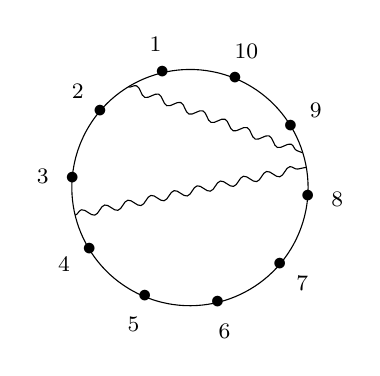
\begin{tikzpicture}[rotate=67.5,baseline=(current bounding box.east)]
	 \begin{scope}
	\drawWLD{10}{1.5}
	\drawnumbers
	\drawprop{1}{0}{8}{1}
	\drawprop{3}{0}{8}{-1}
		\end{scope}
	\end{tikzpicture} \quad ; \quad \textrm{Config 2} = 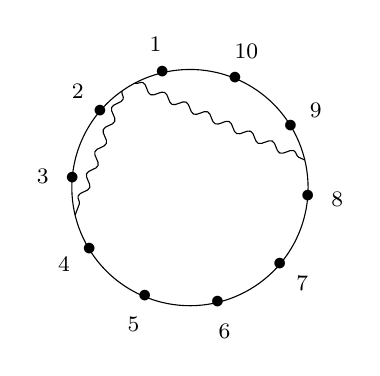
\begin{tikzpicture}[rotate=67.5,baseline=(current bounding box.east)]
	\begin{scope}
	\drawWLD{10}{1.5}
	\drawnumbers
	\drawprop{1}{-1}{8}{0}
	\drawprop{1}{1}{3}{0}
		\end{scope}
	\end{tikzpicture} \\ \textrm{Config 3} = 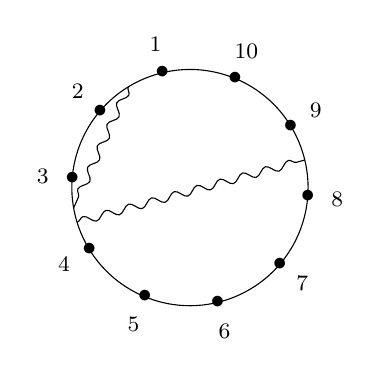
\begin{tikzpicture}[rotate=67.5,baseline=(current bounding box.east)]
	\begin{scope}
	\drawWLD{10}{1.5}
	\drawnumbers
	\drawprop{1}{0}{3}{-1}
	\drawprop{3}{1}{8}{0}
		\end{scope}
	\end{tikzpicture}\emls 

\begin{lem}
Let $W_1$, $W_2$ and $W_3$ be admissible Wilson loop diagrams that are identical except for the fact that the diagram $W_i$ cotains the pair of adjascent propagators shown in $\textrm{Config i}$ above. Then 
\bas \sum_{i = 1}^3 \lim_{\textrm{degree 2 factor of } R(W_i) \rightarrow 0} I(W_i) = 0\;.\eas \end{lem}

This proof is also given in \cite{HeslopStewart, casestudy} but is included here for completeness.
\begin{proof}
Without loss of generality, write $(C_*(W_i))$ with the pertinent propagators represented in the first two rows. Then the matrices $C_*(W_i)$ are identical except for the first two rows. Since the propagators are adjacent, by Lemma \ref{lem:simplifyR(W)} we may write the first two rows as \bas C_*(W_1) = \begin{bmatrix}1 & \ldots & a &b &\ldots & 0 & 0 & \ldots & c & d   \ldots\\  1 & \dots &  ae &be + f  & \ldots &g & h & \ldots &0 &0  \ldots   \end{bmatrix}  \\ C_*(W_2) = \begin{bmatrix}1 & \ldots & a' & b' &\ldots & c' & d' & \ldots & 0 & 0   \ldots\\  1 & \dots &  0 & 0  & \ldots &c'e' & d' e' + f' & \ldots &g' &h'  \ldots   \end{bmatrix} \\C_*(W_3) = \begin{bmatrix}1 & \ldots & 0 &0 &\ldots & a'' & b'' & \ldots & c'' & c''   \ldots\\  1 & \dots &  e'' & f''  & \ldots &0 & 0 & \ldots &c''g'' & d'' g'' + h'' \ldots   \end{bmatrix}\;.\eas We multiple the first two rows of $C_*(W_2)$ and $C_*(W_3)$ by elements of $GL(2)$, leaving the rest of the rows unchanged. Namely, consider the products: \bas \begin{bmatrix} \frac{- e'}{1-e'} & \frac{1}{1-e'} \\ 1 & 0  \end{bmatrix} C_*(W_2) = \begin{bmatrix}  1 & \dots & \frac{-e' a'}{1- e'}  & \frac{-e' b'}{1- e'}  & \ldots &0 & \frac{ f'}{1-e'} & \ldots &\frac{g'}{1-e'} &\frac{h'}{1-e'}  \ldots  \\ 1 & \ldots & a' & b' &\ldots & c' & d' & \ldots & 0 & 0   \ldots \end{bmatrix}  \\ \begin{bmatrix}  \frac{1}{1-c''} & \frac{-c''}{1-c''}\\ 0  & 1  \end{bmatrix} C_*(W_3) = \begin{bmatrix}1 & \ldots & \frac{-e''c''}{1-c''} &\frac{-f''c''}{1-c''} &\ldots & a'' & b'' & \ldots & 0 & \frac{d''}{1-c''}   \ldots\\  1 & \dots &  e'' & f''  & \ldots &\frac{a''}{1-c''} & \frac{b''}{1-c''} & \ldots &g'' & h'' \ldots   \end{bmatrix}\;.\eas
From this, we see that, in the limit $f \rightarrow 0$ and $f' \rightarrow 0$, for $C_*(W_2)$, we have the change of variables \bmls a = \frac{-e'a'}{1-e'} \quad ; \quad b = \frac{-e'b'}{1-e'} \quad ; \quad c = \frac{g'}{1-e'} \quad ; \quad d = \frac{d}{1-e'}  \quad ; \\ \quad e = \frac{1-e'}{e'}\quad ; \quad f = 0 \quad ; \quad g = c' \quad ; \quad h = d'\;.\emls Inverting and performing the change of variables, we see that $\lim_{f' \rightarrow 0} I(W_2) = \lim_{f \rightarrow 0} \frac{1}{1-e} I(W_1)$. A similar calculation shows that $\lim_{d'' \rightarrow 0} I(W_3) = \lim_{f \rightarrow 0} \frac{-1}{1-e} I(W_1)$. Thus, in the appropriate limit, \bas \lim_{f \rightarrow 0} I(W_1) + \lim_{f' \rightarrow 0} I(W_2) + \lim_{d'' \rightarrow 0} I(W_3) = 0\;.\eas  \end{proof} \todo{actually check these calculations, minus signs, etc.}

The last case to consider consists of understanding the poles shared between the diagrams with the following configureations: \bmls \textrm{Config 4} = 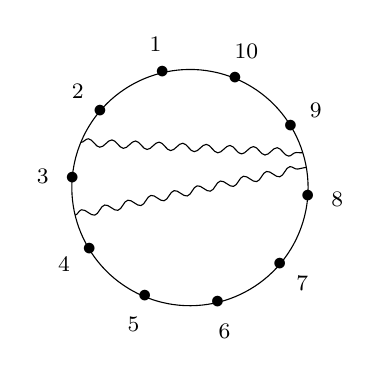
\begin{tikzpicture}[rotate=67.5,baseline=(current bounding box.east)]
	 \begin{scope}
	\drawWLD{10}{1.5}
	\drawnumbers
	\drawprop{2}{0}{8}{1}
	\drawprop{3}{0}{8}{-1}
		\end{scope}
	\end{tikzpicture} \quad ; \quad \textrm{Config 5} = 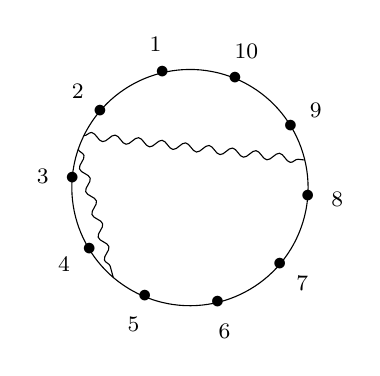
\begin{tikzpicture}[rotate=67.5,baseline=(current bounding box.east)]
	\begin{scope}
	\drawWLD{10}{1.5}
	\drawnumbers
	\drawprop{2}{-1}{8}{0}
	\drawprop{2}{1}{4}{0}
		\end{scope}
	\end{tikzpicture} \\ \textrm{Config 6} = 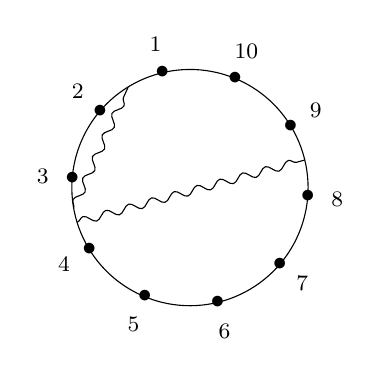
\begin{tikzpicture}[rotate=67.5,baseline=(current bounding box.east)]
	\begin{scope}
	\drawWLD{10}{1.5}
	\drawnumbers
	\drawprop{3}{1}{8}{0}
	\drawprop{3}{-1}{1}{0}
		\end{scope}
	\end{tikzpicture}\emls 

\begin{lem}
Let $W_4$, $W_5$ and $W_6$ be admissible Wilson loop diagrams that are identical except for the fact that the diagram $W_i$ cotains the pair of propagators shown in $\textrm{Config i}$ above. Let $p = (i, j)$ and $q = (i, k)$ with $k = j+1$. Then \bas \lim_{(c_{p,i}c_{q, i+1} - c_{p, i+1}, c_{q, i}) \rightarrow 0} I(W_4) + \lim_{c_{r, j+3} \rightarrow 0}I(W_5) + \lim_{c_{r, k-2} \rightarrow 0}I(W_6) = 0\;.\eas \end{lem}
\begin{proof}
This proof follows similarly to the above. Write \bas C_*(W_4) = \begin{bmatrix}1 & \ldots & a &b &\ldots & c & d & 0 & \ldots \\  1 & \dots &  ae &be + f  & \ldots &0 & g & h & \ldots    \end{bmatrix}  \\ C_*(W_5) = \begin{bmatrix}1 & \ldots & a' &b' &\ldots & c' & d' & 0 & 0& \ldots \\  1 & \dots &  0&0  & \ldots &c'e' & d'e' +f' & g' & h' & \ldots    \end{bmatrix} \\ C_*(W_6) = \begin{bmatrix}1 & \ldots & 0 &0 &\ldots & a'' & b'' & c''g'' & h'' c'' + d'' & \ldots \\  1 & \dots &  e'' & f''  & \ldots &0&0 & g'' & h'' & \ldots    \end{bmatrix} \;. \eas We consider the change of variables defined by the product \bas \begin{bmatrix}1 & 0 \\ \frac{-e'}{1-e'} & \frac{1}{1-e'} \end{bmatrix} C_*(W_5)  \quad \textrm{ and } \quad \begin{bmatrix}\frac{1}{1-c''} & \frac{-c''}{1-c''} \\ 0 & 1 \end{bmatrix} C_*(W_6) \;.\eas Then the same types of calculations as in Lemma \ref{??} shows that $ \lim_{c_{r, k-2} \rightarrow 0}I(W_6)  =  \lim_{f \rightarrow 0} \frac{-1}{1-e} I(W_4) $ and $\lim_{c_{r, k-2} \rightarrow 0}I(W_5)  =  \lim_{f \rightarrow 0} \frac{e}{1-e} I(W_4) $, proving the result.
\end{proof}

\begin{thm}
Let $\mathbf{p} = p_1, p_2, \dots, p_d$ be algebraically independent invertible variables and let $C(\mathbf{p})$ be a $n \times k$ matrix with entries in $\mathbb{R}(\mathbf{p})$.
Let $R_i$ be the $i^{th}$ row of $C(\mathbf{p})$. SOME HYPOTHESIS ABOUT NOT HAVING A SILLY OVER PARAMETERIZATION JUST WITHIN A ROW. Let $G(C(\mathbf{p}))$ be the subset of $\Gr(k,n)$ consisting of row spaces of matrices obtained by evaluating the parameters of $C(\mathbf{p})$ at real entries. The following are equivalent:
\begin{itemize}
\item[(i)] For all $I \subseteq \{1,2, \dots, k\}$ and all $j \notin I$,
\begin{displaymath}
\mathrm{span} \left( \bigcup_{i \in I} R_i \right)
\neq \mathrm{span} \left( \bigcup_{i \in I \cup j} R_i \right),
\end{displaymath}
\noindent
where spans are taken in $(\mathbb{R}(\mathbf{p}))^n$.
\item[(ii)] $\mathrm{dim} (G(C(\mathbf{p}))) = d$.
\end{itemize}
\end{thm}

Theorem XX in \cite{basisshapeloce} gave a formula
\begin{proof}
\end{proof}

\begin{eg}
Consider
\begin{displaymath}
\begin{bmatrix}
1 & p_1 & p_2 & p_3 & p_4 & 0 & 0 \\
1 & p_1 p_5 & p_2 p_5 + p_6 & 0 & 0 & p_7 & p_8 \\
1 & 0 & 0 & p_9 & p_{10} & p_{11} & p_{12}
\end{bmatrix}
\end{displaymath}
can kill off 9
\end{eg}

\begin{rmk}
remark: this is a rado theorem thing.
\end{rmk}

\end{appendices}








\end{document}
